\chapter{\label{chap:intro}Introdução}

Em 2014, 54\% da população mundial vivia em áreas urbanas, de acordo com a Organização das Nações Unidas (\cite{UN14}). A expectativa é que esta proporção aumente para 66\% até o ano 2050. Em números absolutos isto representa um acréscimo de 2,5 bilhões de pessoas à população urbana mundial nos próximos 35 anos. Uma das consequências da alta densidade populacional em regiões geográficas limitadas é o crescimento do modelo de verticalização na construção civil. Neste cenário, onde prédios de diversos andares se tornam presença no cotidiano da maioria da população, os elevadores passam a um papel de grande destaque.

http://www.bls.gov/news.release/empsit.t19.htm

\begin{figure}[htb!]
\centering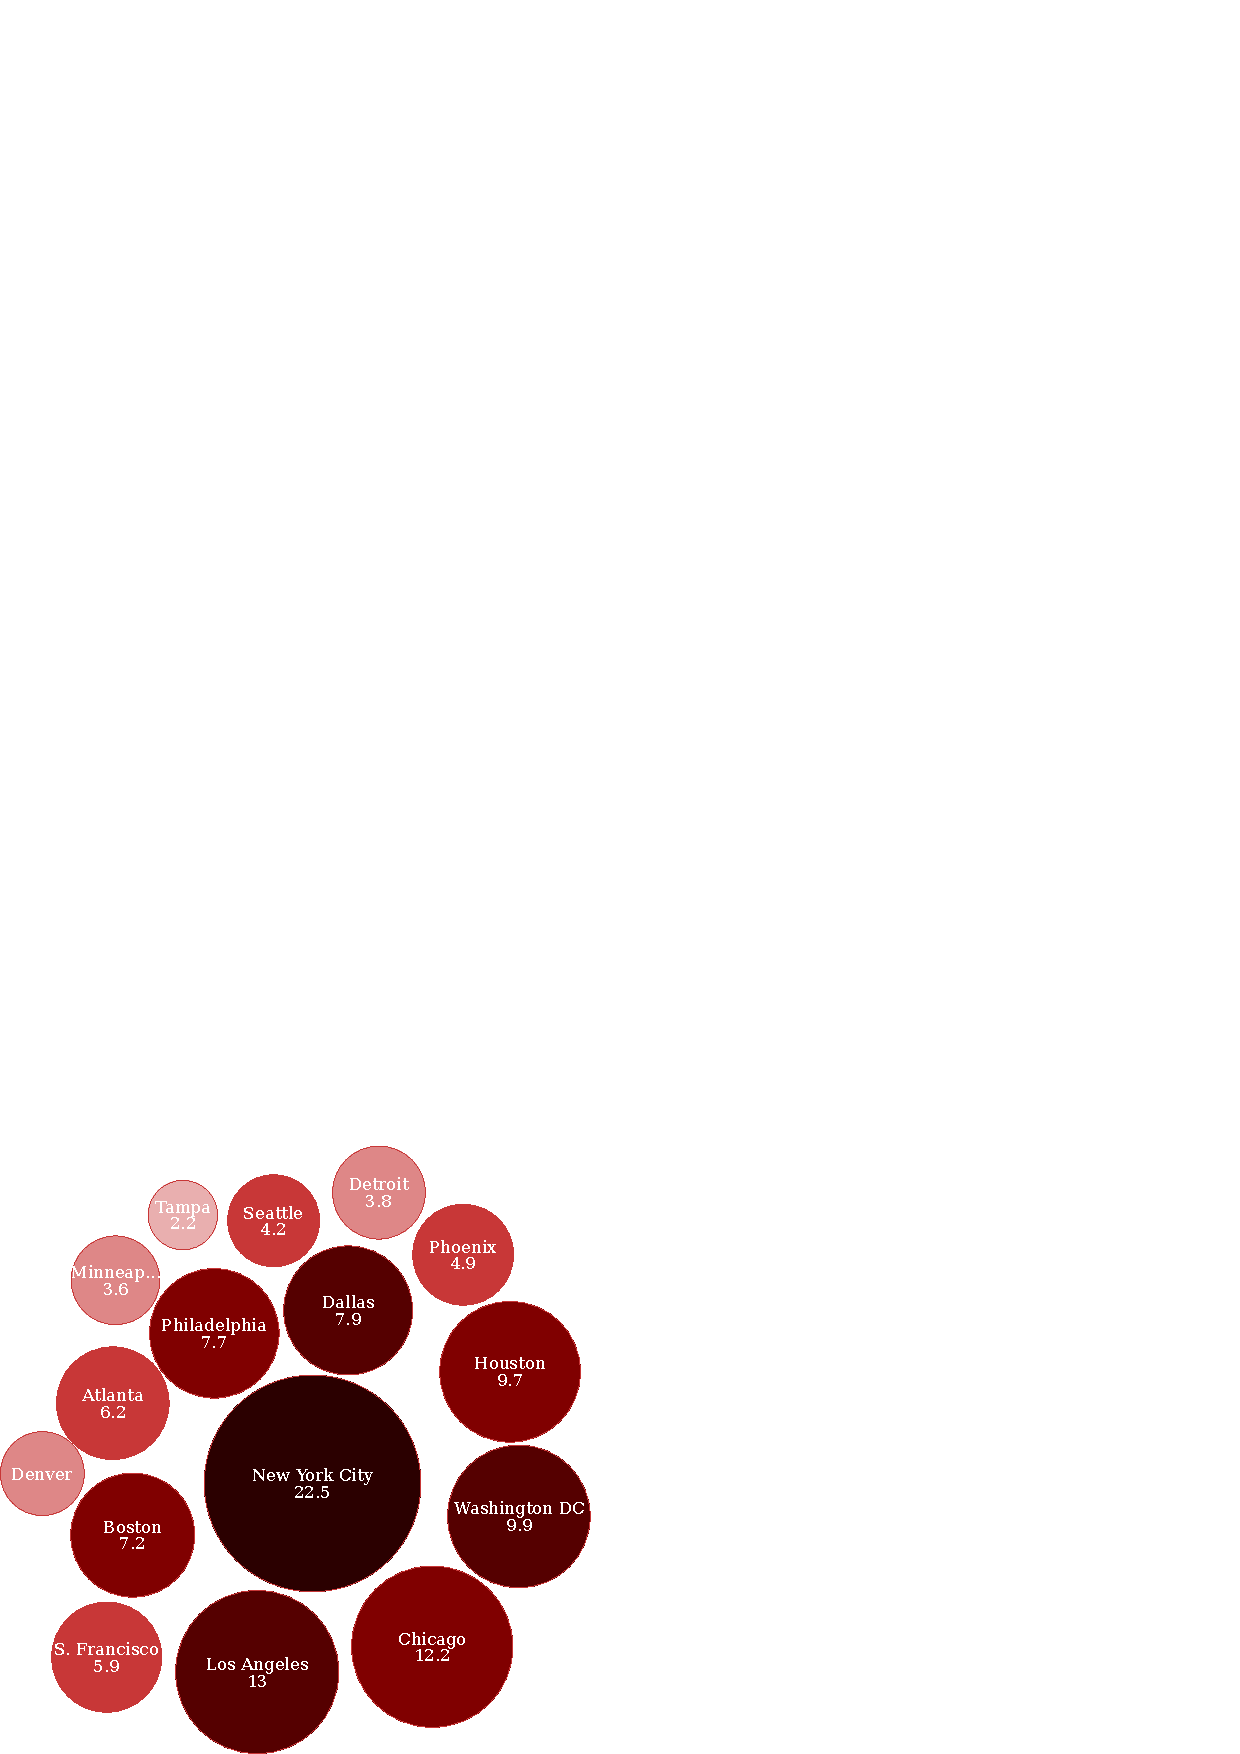
\includegraphics{img/time-cost.jpg}
\caption{\label{fig:fig1}Tempo cumulativo (em anos) que trabalhadores de escritórios gastaram aguardando elevadores durante 12 meses em 16 cidades norte-americanas. Fonte:\cite{Horn10}}
\end{figure}

\cite{Sharma12}

\section{Motivação prática}
\section{Testar conhecimentos}
\subsection{IA}
\subsection{Programação}
\section{Simulação}